\documentclass[../Head/report.tex]{subfiles}
\begin{document}
\section{Methods}
\label{sec:methods}

This section is about the used methods in regards to 3D models, simulation environments, navigation control, general theory for the pose estimation of ArUco markers and setup of the drone to utilize autonomous flight.

The methods used will follow the general time schedule defined in the introduction where the project has been split up into two major parts i.e. the implementation and simulations of the drone in Gazebo, and real life flight of the drone in Hans Christian Andersen Airport in Odense using the PX4 flight controller and a Raspberry pi for pose estimation with autonomous execution using robot operating system (ROS) as the main target.

\subsection{3D modeling for Gazebo simulations}

This section will go through the models created and why they were considered to be important for properly testing the system before real life implementations on the drone. Moreover, the simulation environment Gazebo will be discussed and how the 3D models have been imported into this software.     

\label{sec:3d_modeling_for_gazebo_simulations}
\subsubsection{3D modeling}
The models have been created using the 3D modeling software Blender. This is an open source software used on Ubuntu which is the operating system used. In the modeling software, the ArUco markers can be imported as images as planes and the final model saved as a \textit{.dae} file which is easily imported in a simulator software like Gazebo.    

Four different 3D models have been created to be used in the simulation environment as seen in Figures \ref{fig:one_pattern_aruco_fig}, \ref{fig:two_pattern_aruco_fig}, \ref{fig:three_pattern_aruco_fig} and \ref{fig:three_pattern_aruco_error_fig}. Since the actual evaluation of the performance of the drone is to be done in the optitrack system in the airport in Odense, a model of this system has been used with the actual dimensions of the real system. The is done so the pose estimation of the    ArUco markers can be compared to that of the optitrack system which got a millimeter precision in regard to tracking the drone. Hence, the model has been created with these considerations in mind which had put a threshold to the size of the model, which has to fit inside the optitrack system as seen in Figure \ref{fig:optitrack_one_pattern_aruco}. 

The general idea behind this design is that the drone can fly towards the wall and locate the ArUco marker placed at the top of the wall. This will enable GPS to vision based navigation where the drone shifts between using the GPS as the global coordinate system to that of the ArUco markers (vision based). When the drone has positioned itself with a certain distance away from this marker board, it will switch to using the bottom camera where the ArUco board located on the ground will function as a  world coordinate system. In this scenario, the drone is to land on one of three different locations in front of the ArUco board located at the end of each track. Here transformations of the pose of these three ArUco boards have been performed to align these with that of the ArUco board located on the ground (world coordinate) to avoid switching between different coordinate systems. This is because the controller in the PX4 becomes unstable when giving vision coordinates with a very high variance. This will be explained further in Section \ref{sec:px4_autopilot}. 

\begin{figure}[H]
    \centering
    \begin{subfigure}[t]{.48\textwidth}
        \centering
        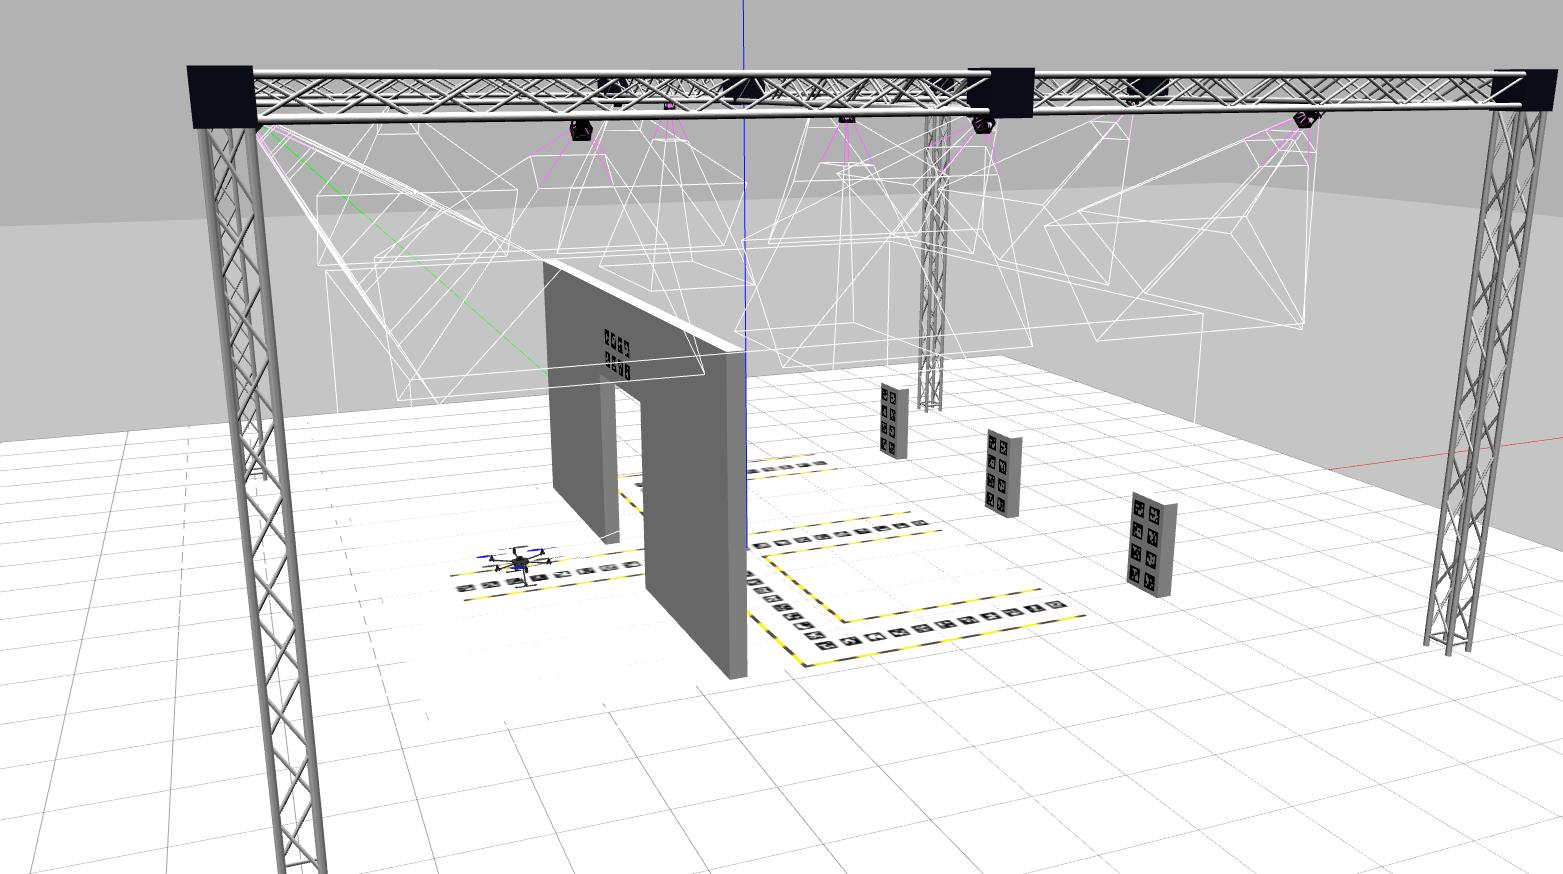
\includegraphics[width=\textwidth]{../Figures/gazebo_one_pattern_view.jpg}
        \caption{}
        \label{fig:optitrack_one_pattern_aruco}
    \end{subfigure}
    \hfill
    \begin{subfigure}[t]{.48\textwidth}
        \centering
        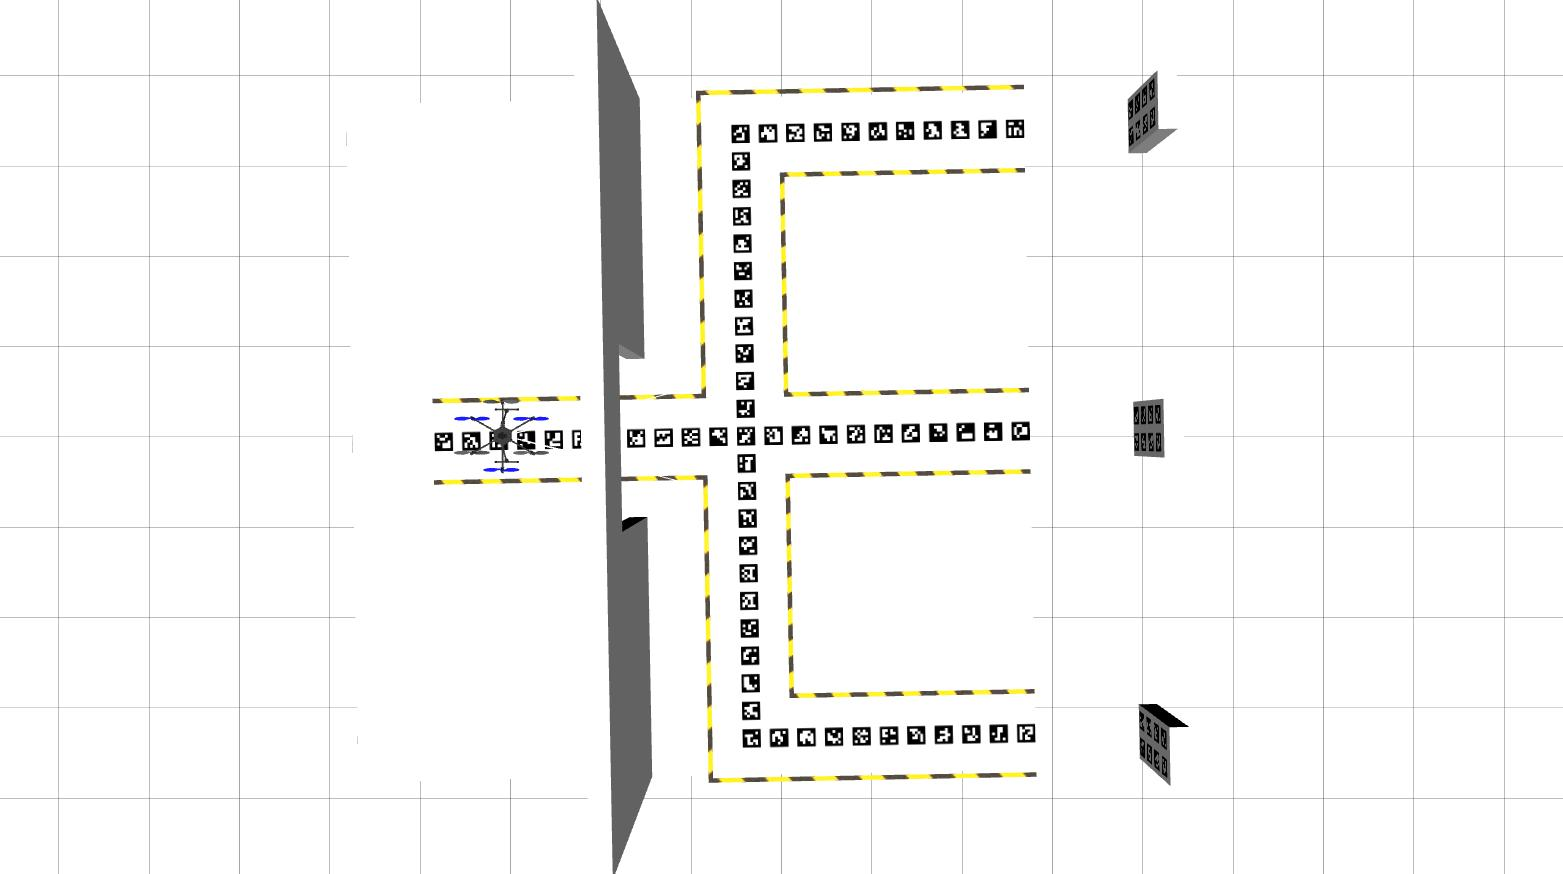
\includegraphics[width=\textwidth]{../Figures/gazebo_one_pattern.jpg}
        \caption{}
        \label{fig:one_pattern_aruco}
    \end{subfigure}
    \caption{Visualisation of the optitrack model in Figure \ref{fig:optitrack_one_pattern_aruco} and top view of the one pattern ArUco marker in Figure \ref{fig:one_pattern_aruco}}
    \label{fig:one_pattern_aruco_fig}
\end{figure}

The ArUco markers used in these models will be ($5 \times 5$) bit markers. The GPS to vision marker board located on the top of the wall will be a ($2\times
4$) with marker length of 0.2 m and marker separation of 0.1 m, the ground marker a ($25\times25$) with marker length of 0.2 m and marker separation of 0.1 m and the landing markers ($4\times2$) with marker length of 0.2 m and marker separation of 0.1 m. These sizes have been chosen to be appropriate taken a flying height of approximately 1.5 m into account based on tests where the pose estimation of the ArUco markers has been found for different flying heights along with the resolution of the camera. These parameters have shown to have a significant impact on the pose estimation which will be analyzed in Section \ref{sec:results}. \todo{Talk more precisely about the tests which have been done to make this evaluation. How many test, under which conditions etc. This goes for all sub chapters in the sections}

If this setup were to be implemented in real life, an implementation with fewer ArUco markers would be beneficial if this would not decrease the precision of the pose estimation too much. In this small ($25\times25$) bit scenario it would not be a general problem, but if this has to be scalable e.g. big industrial companies, great performance using a small amount of ArUco markers would be preferred.
Because the precision of the ArUco pose estimation will be based on the number of ArUco markers located in the image \cite{DetectionOfArUcoBoards}, the estimation of the pose will be based on a full ($25\times25$) ArUco board and a one and three pattern setup as seen in Figure \ref{fig:full_pattern_aruco}, \ref{fig:one_pattern_aruco} and \ref{fig:three_pattern_aruco} respectively. The performance of these different setups will be evaluated where the drone is starting from the position illustrated in \ref{fig:optitrack_three_pattern_aruco}, takes off and moves to one of the landing locations. The outcome of this will be compared between the three models along with the error in the pose estimation. This will be analyzed in Section \ref{sec:results}.      

\begin{figure}[H]
    \centering
    \begin{subfigure}[t]{.48\textwidth}
        \centering
        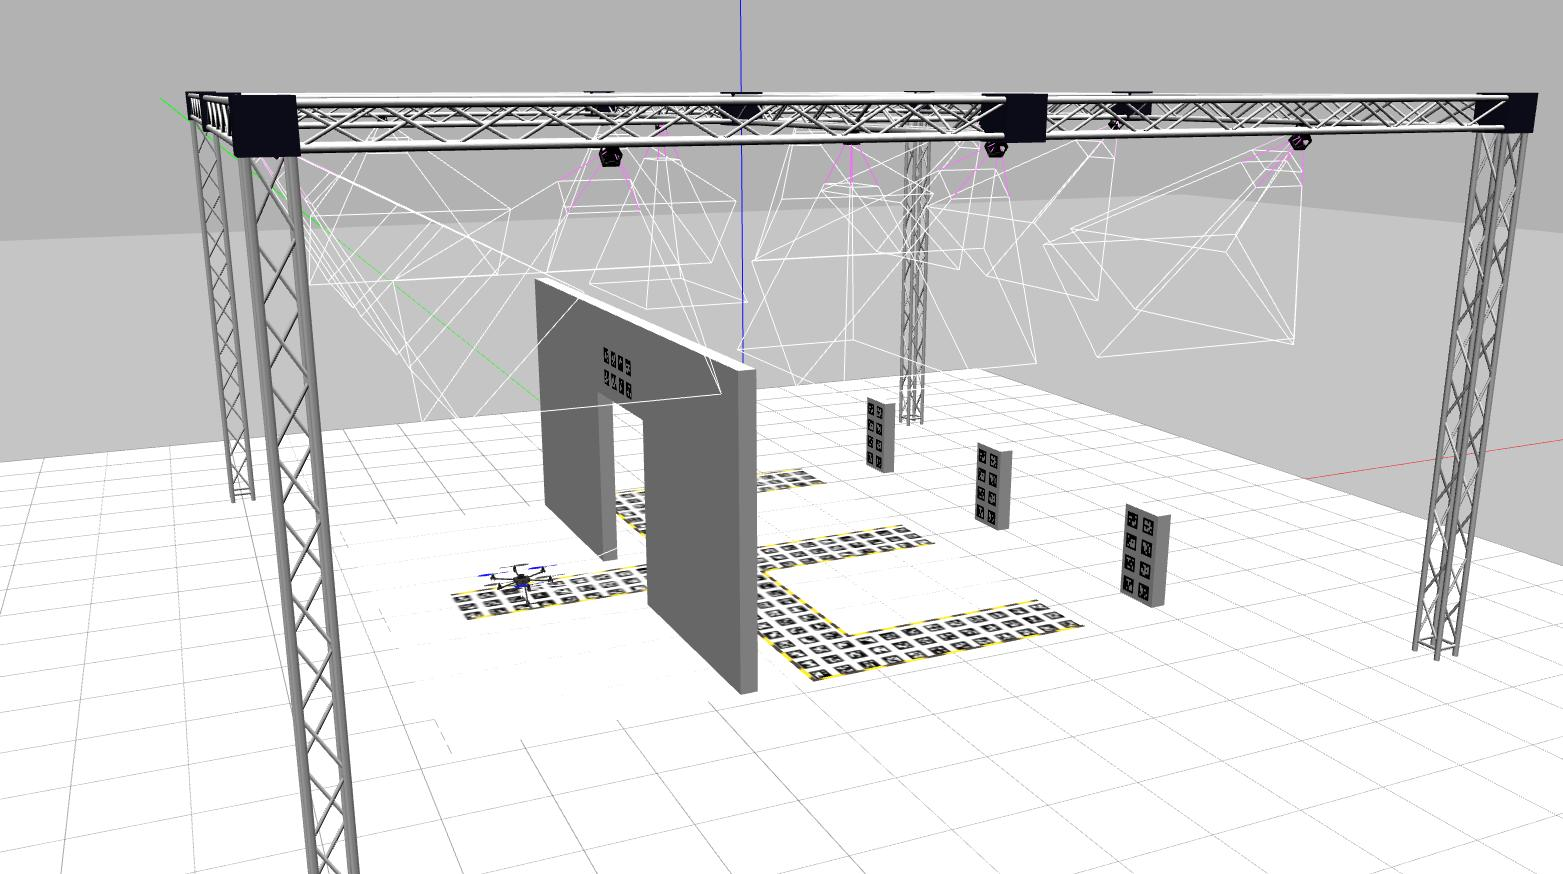
\includegraphics[width=\textwidth]{../Figures/gazebo_three_pattern_view.jpg}
        \caption{}
        \label{fig:optitrack_three_pattern_aruco}
    \end{subfigure}
    \hfill
    \begin{subfigure}[t]{.48\textwidth}
        \centering
        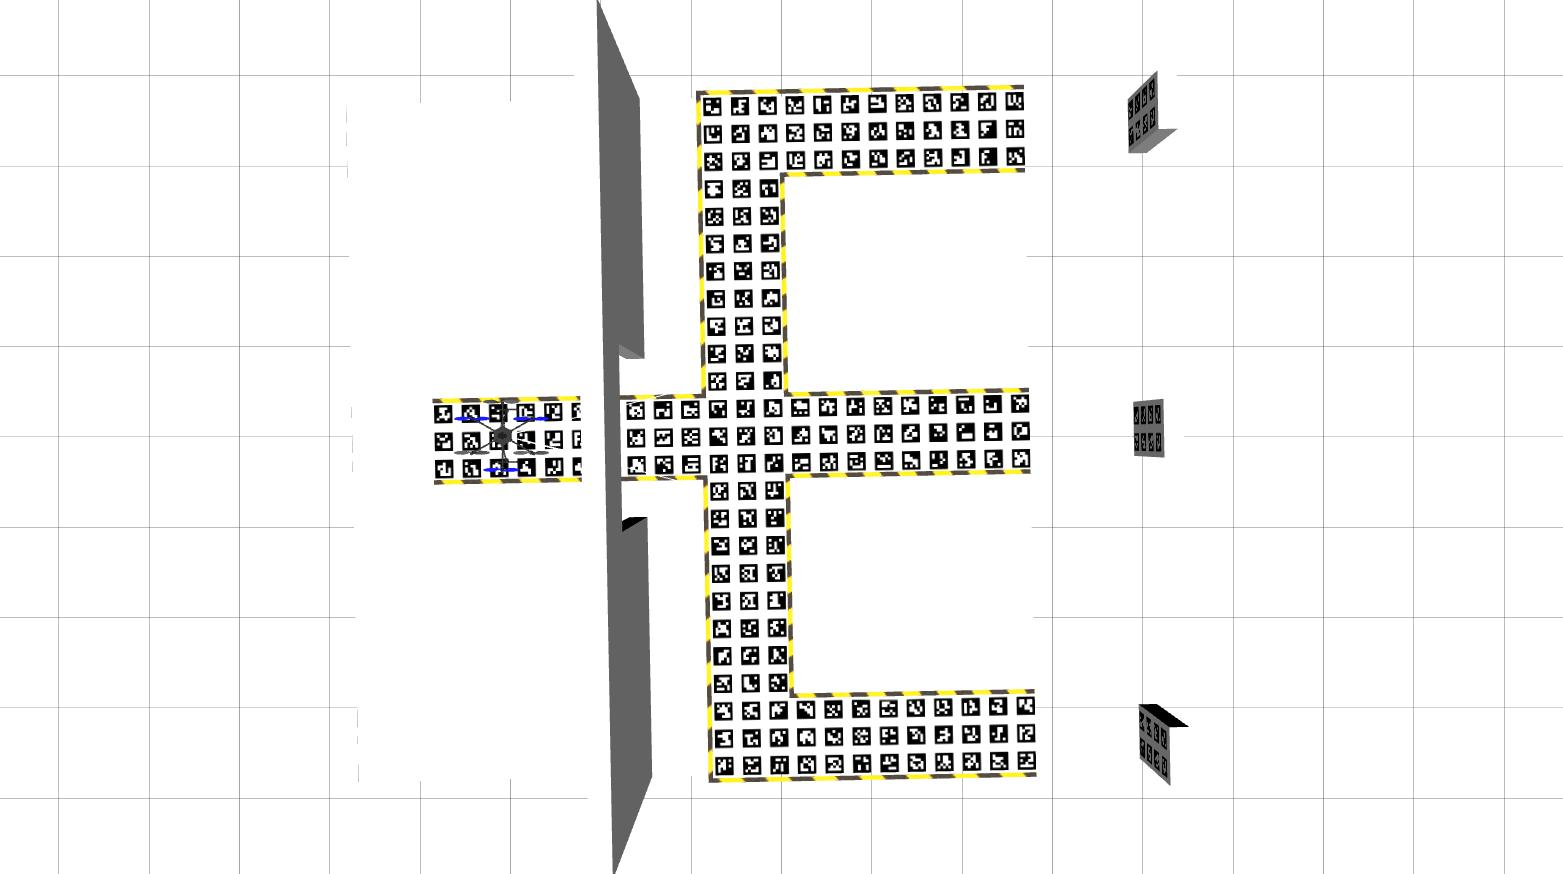
\includegraphics[width=\textwidth]{../Figures/gazebo_three_pattern.jpg}
        \caption{}
        \label{fig:three_pattern_aruco}
    \end{subfigure}
    \caption{Visualisation of the optitrack model in Figure \ref{fig:optitrack_three_pattern_aruco} and top view of the three pattern ArUco marker in Figure \ref{fig:three_pattern_aruco}}
    \label{fig:two_pattern_aruco_fig}
\end{figure}

\begin{figure}[H]
    \centering
    \begin{subfigure}[t]{.48\textwidth}
        \centering
        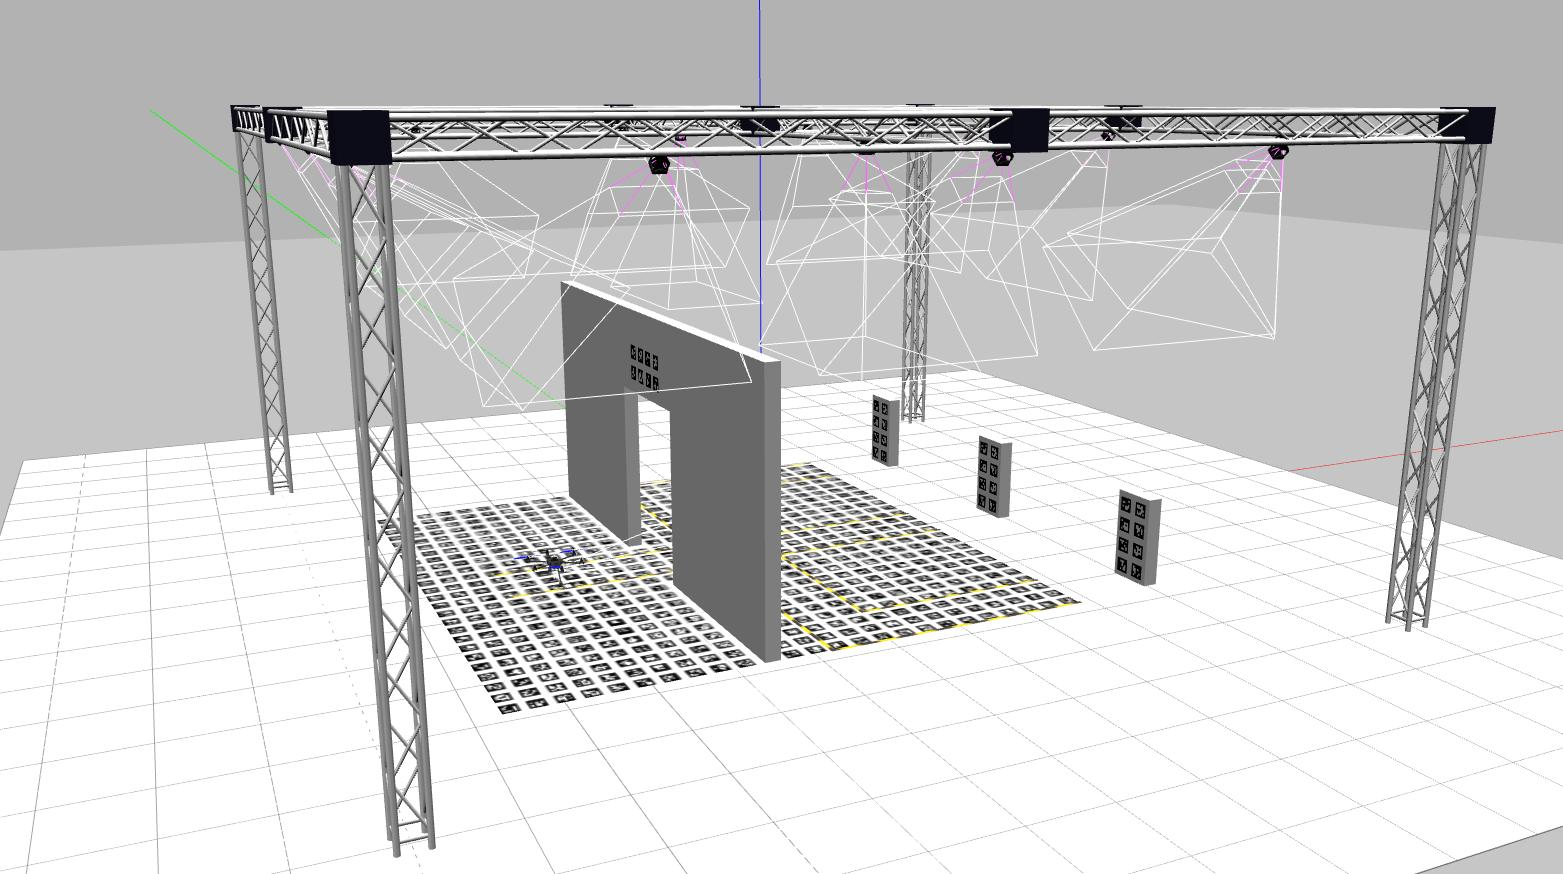
\includegraphics[width=\textwidth]{../Figures/gazebo_full_pattern_view.jpg}
        \caption{}
        \label{fig:optitrack_full_pattern_aruco}
    \end{subfigure}
    \hfill
    \begin{subfigure}[t]{.48\textwidth}
        \centering
        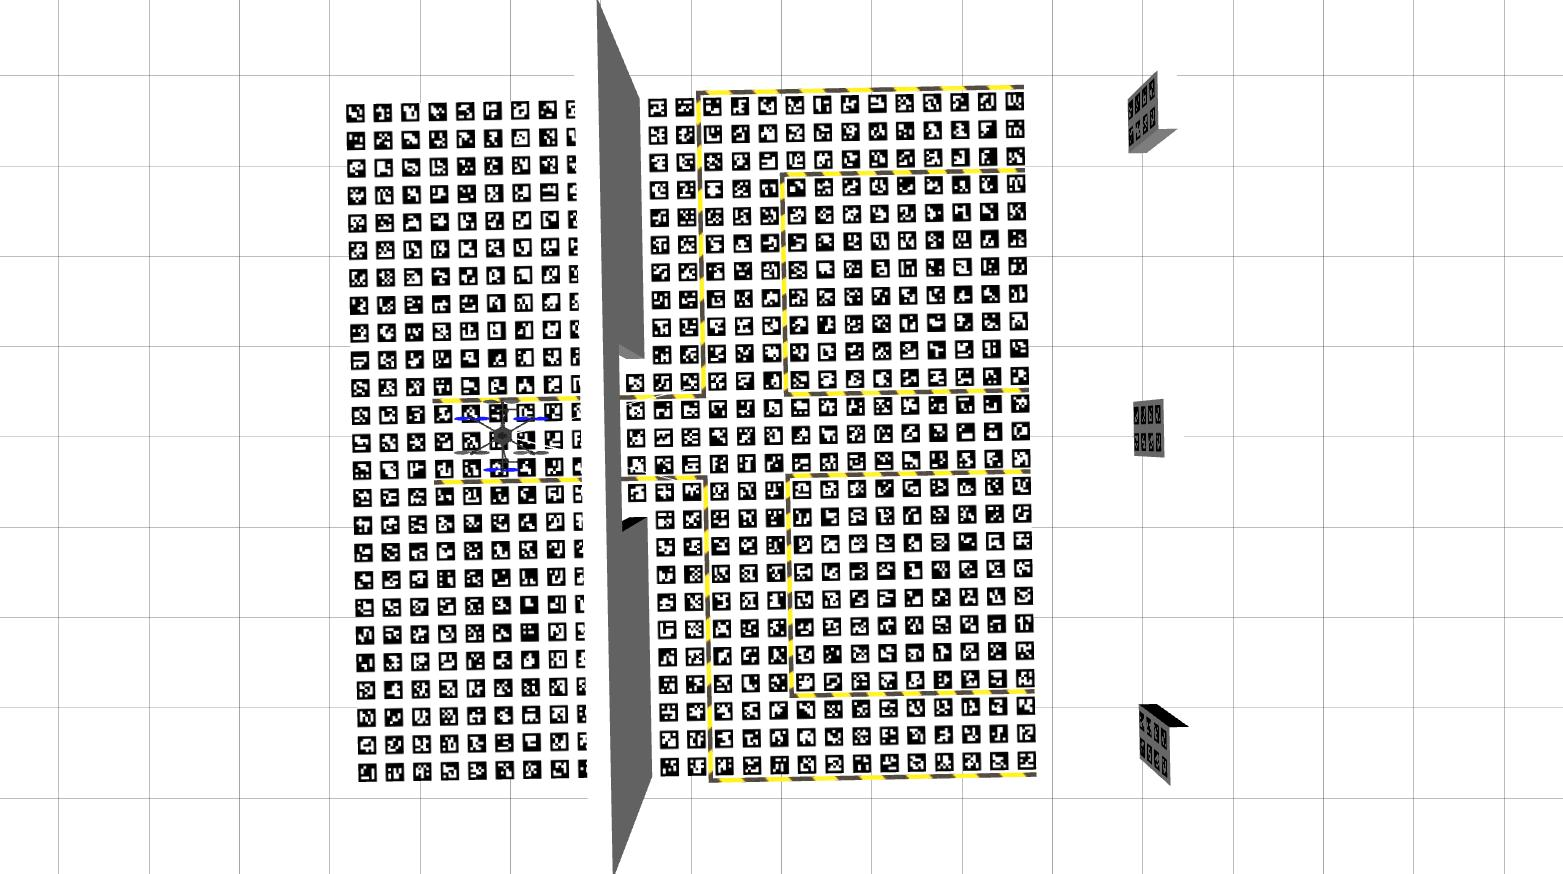
\includegraphics[width=\textwidth]{../Figures/gazebo_full_pattern.jpg}
        \caption{}
        \label{fig:full_pattern_aruco}
    \end{subfigure}
    \caption{Visualisation of the optitrack model in Figure \ref{fig:optitrack_full_pattern_aruco} and top view of the full pattern ArUco marker in Figure \ref{fig:full_pattern_aruco}}
    \label{fig:three_pattern_aruco_fig}
\end{figure}

Because relying completely on vision based navigation will put the system in a vulnerable position e.g. no markers are found in the image, optimizations have to be performed. This will be utilized through sensor fusion where the pose estimation from the ArUco markers, drone acceleration and angular velocity from the accelerometer and gyro (Inertial measurement unit) will be fused together to give a more reliable estimation of the current position of the drone. To evaluate the performance of sensor fusion, a model with missing ArUco markers has been created as seen in Figure \ref{fig:three_pattern_aruco_error_fig}. The goal of this is to have the drone to fly a couple of meters without any global position (vision) for the pose estimation and still keeps its track until the pose will be updated when markers again is visible for the drone. More of the implementation of this in Section \ref{sec:sensor_fusion_for_pose_optimization}. 

When operating in real life scenarios, a clean image without any noise is rarely seen. To take this into account, the ($25\times25$) ground marker will be added noise like Gaussian noise, custom rain, snow and fog to illustrate real life conditions \cite{imgaug}. This is used to stress test the system and see how the pose estimation of the ArUco markers will perform under hard conditions. Illustrations of such noisy environments can be seen in Figure \ref{fig:added_fog_one_pattern_aruco_fig}. Here the evaluations will be based on the one pattern ArUco marker where the noise added images are used in the simulations and compared to those without any noise.      

\begin{figure}[H]
    \centering
    \begin{subfigure}[t]{.48\textwidth}
        \centering
        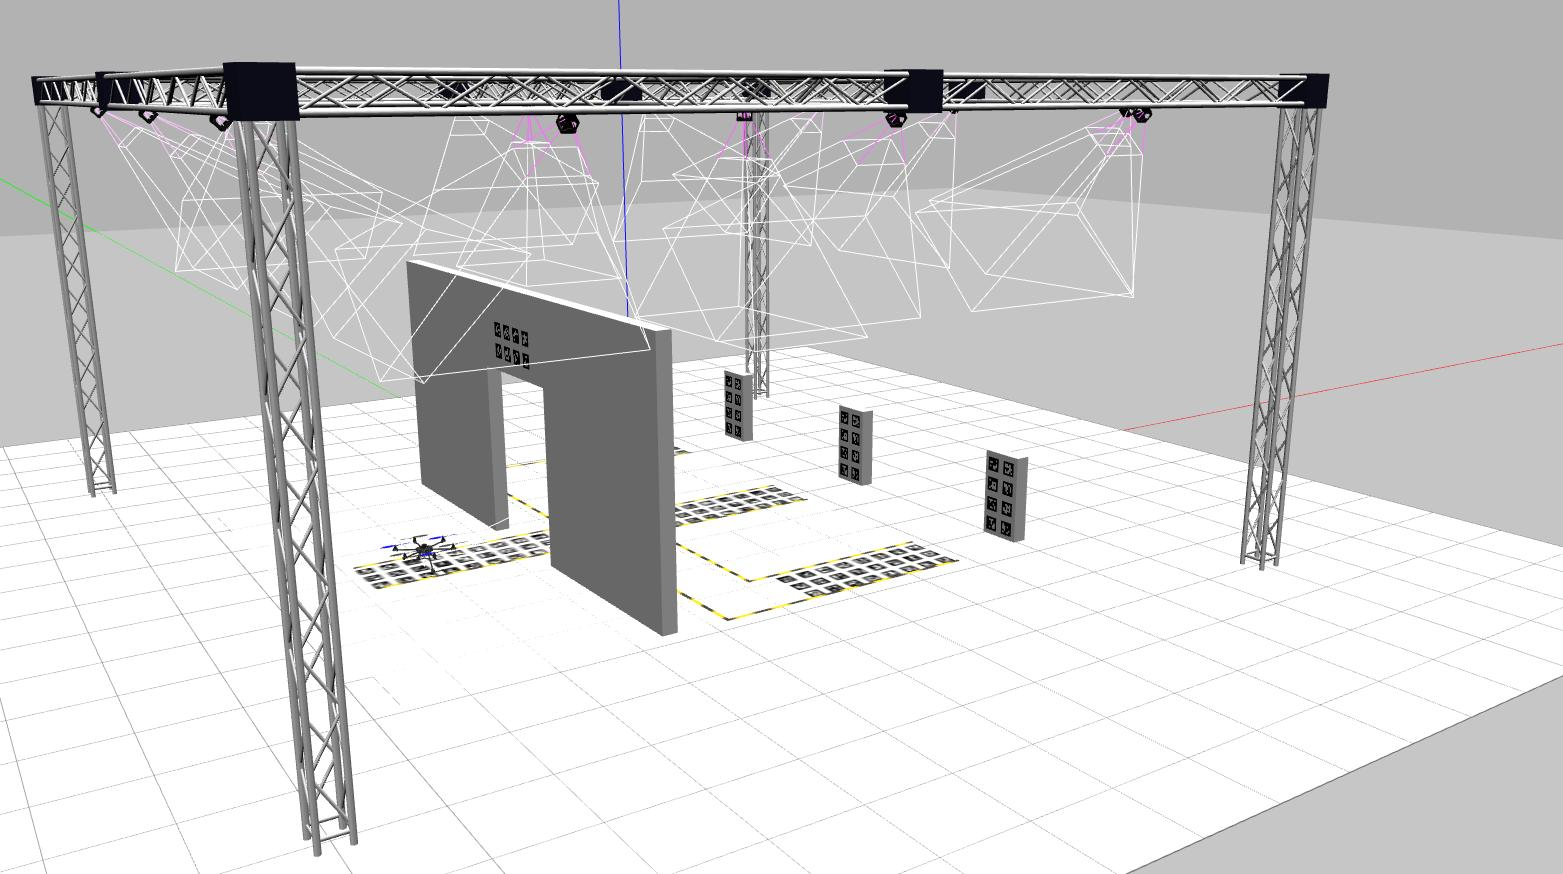
\includegraphics[width=\textwidth]{../Figures/gazebo_three_pattern_error_view.jpg}
        \caption{}
        \label{fig:optitrack_three_pattern_aruco_error}
    \end{subfigure}
    \hfill
    \begin{subfigure}[t]{.48\textwidth}
        \centering
        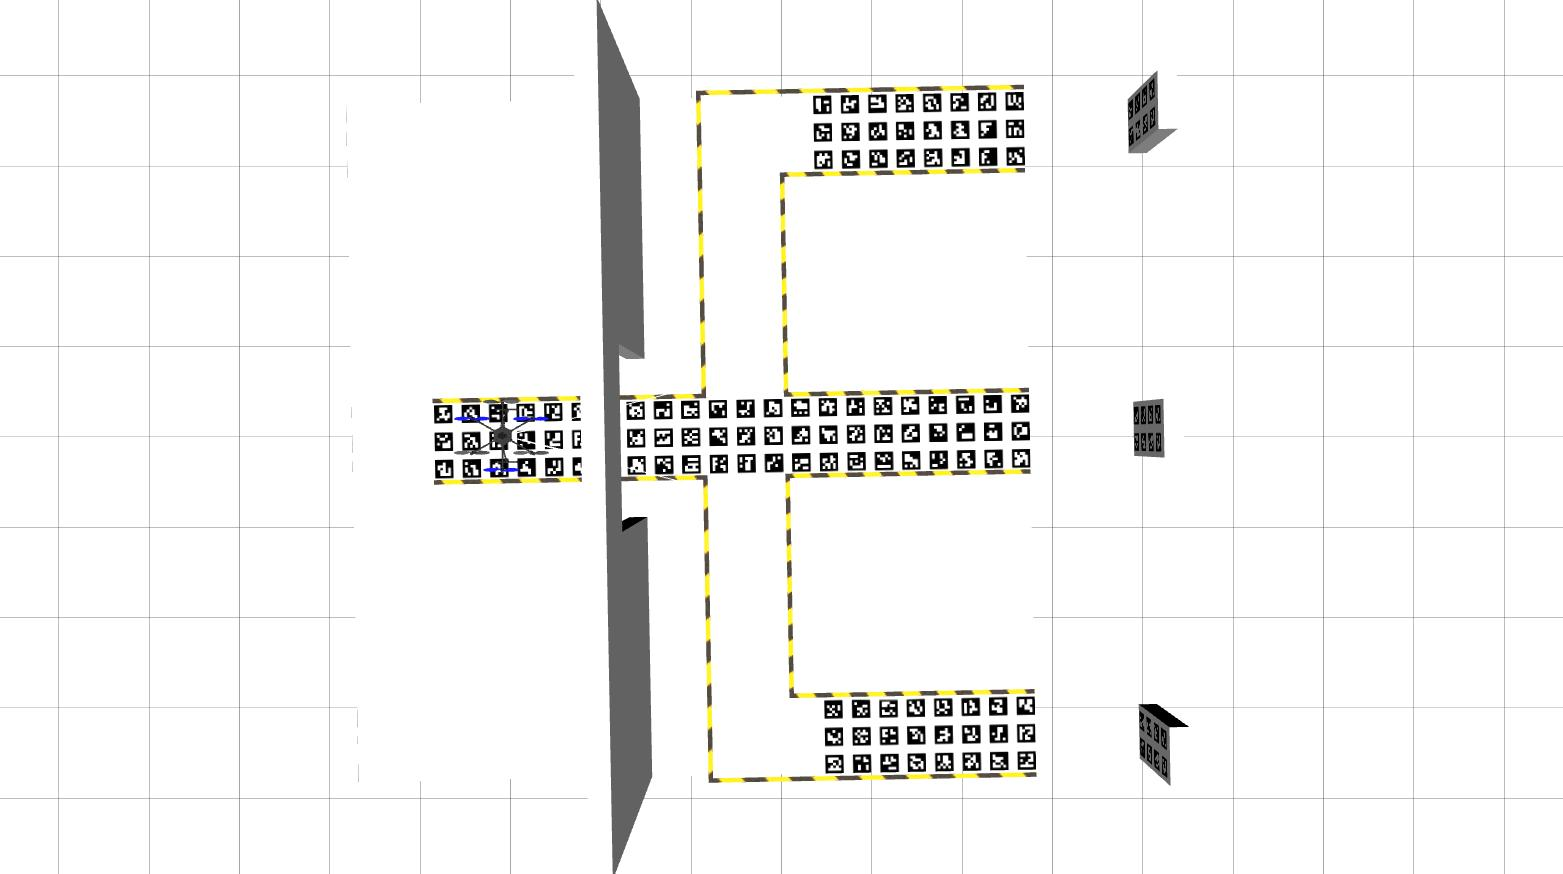
\includegraphics[width=\textwidth]{../Figures/gazebo_three_pattern_error.jpg}
        \caption{}
        \label{fig:three_pattern_aruco_error}
    \end{subfigure}
    \caption{Visualisation of the optitrack model in Figure \ref{fig:optitrack_three_pattern_aruco_error} and top view of the three pattern ArUco marker with errors in Figure \ref{fig:three_pattern_aruco_error} to be used for testing the implementation of sensor fusion}
    \label{fig:three_pattern_aruco_error_fig}
\end{figure}

\begin{figure}[H]
    \centering
    \begin{subfigure}[t]{.34\textwidth}
        \centering
        \includegraphics[width=\textwidth]{../Figures/one_pattern_aruco_noise1.png}
        \caption{}
        \label{fig:added_noise_one_pattern_aruco}
    \end{subfigure}
      \hskip 15ex
    \begin{subfigure}[t]{.34\textwidth}
        \centering
        \includegraphics[width=\textwidth]{../Figures/one_pattern_aruco_noise3.png}
        \caption{}
        \label{fig:added_fog_one_pattern_aruco}
    \end{subfigure}
    \caption{Examples of added noise like Gaussian blur, Gaussian noise, custom fog, rain and snow to illustrate real life scenarios which can be seen in Figure \ref{fig:added_noise_one_pattern_aruco} and \ref{fig:added_fog_one_pattern_aruco} for stress testing of the ArUco pose estimation}
    \label{fig:added_fog_one_pattern_aruco_fig}
\end{figure}

\todo{talk about which kinds of noise has will be added and how many tests are performed. Consider to use some kind of average performance for the specific kind of noise in the image - maybe the systems performs better which Gaussian noise than fog. Make tables for inference of the required data. }

\subsubsection{Gazebo simulator}
\label{sec:gazebo}

Gazebo is an open source 3D robotic simulator which integrates the open dynamics engine (ODE) physics engine, openGL rendering and supports code for both actuator control and sensor simulation. Using this software, the drone can be tested and simulated in environments and conditions close to real life. Hence, all tests will be performed in simulation before further action will be executed with the drone. Furthermore, wind can be applied to the simulation which will also be a critical aspect to consider before deployment of the drone. 

To use the newly created models, a world file must be defined. The world file includes all elements which are to be included in a given simulation such as robots, lights, sensors, objects etc. The file must end with a \textit{.world} extension to be recognized as a world file. The GZServer will read this file which builds the world as a virtual environment for which the robot can operate. This means that the operation can be visualized using GZClient or be run in the background only using GZServer to save systems resources. The latter corresponds to running Gazebo in headless mode, which is a great feature to use if a number of simulations have to be performed in a automatic fashion.

The world file uses the SDF format which contains things like \textit{worlds}, \textit{models} etc. Joints can be set to be either revolute or prismatic according to the wanted configuration. To each joint a link can be attached. The collision, visualization and inertia tags specifies the visualization for the model, collision detection and physics in gazebo respectively. The static tags are used for models which have to be static throughout a simulation like ground, tress etc. The same SDF format is used when creating a model, where the \textit{.dae} file is included to use the 3D models created in Blender.  

The plugins in gazebo are code which is compiled as a shared library and inserted into the simulation. These plugins includes world, model, sensors, system, visual and GUI. For instance, if one wants to include a feature to an existing model, like a wind plugin, these can be included into the world file to be used in a simulation. This wind plugin will be used in some of the simulations for stress testing of the ArUco pose estimation and the flight control in general. \todo{Explain in detail how these wind tests are going to be performed. The wind test is only relevant for the GPS to vision marker and ground marker following. The landing are to be performed in a indoor environment}

\subsection{PX4 and ROS for autonomous flight}

This section deals with the implementation of the autonomous flight of the drone. The PX4 autopilot will be used as flight controller which offers many features to enable autonomous flight. Along the PX4 software, ROS will be used which enables onboard computing on the raspberry pi and transmission of messages to the PX4 using the MAVROS package. Before the setup of the raspberry pi, this onboard computing will be simulated in Gazebo and tested thoroughly before moving further. This leads to the execution of flight plans and actions taking by the drone which will be discussed along the implementation of ROS. 

\subsubsection{PX4 flight stack}
\label{sec:px4_flight_stack}

PX4 is an open source control software for unmanned vehicles. PX4 uses software in the loop (SITL) for simulations of a given unit before real world testing. The flight stack runs on a computer which could be any unit on the same network. Hardware in the loop (HITL) uses simulation software on a real flight controller board e.g PX4 mini which will be the used as flight controller on the drone. 

MAVROS is a packages that provides communication drivers for various autopilots with the MAVLink communication protocol. MAVLink is categorized as a light weight messaging protocol for communication with drones, other unmanned vehicles and there onboard components. This follows a hybrid publish-subscribe and point-to-point design pattern. A visualization of how this works can be seen in Figure \ref{fig:sitl_simulation_enviroment}.   

\begin{figure}[H]
    \centering
    \begin{subfigure}[b]{0.48
    \linewidth}
        \centering
        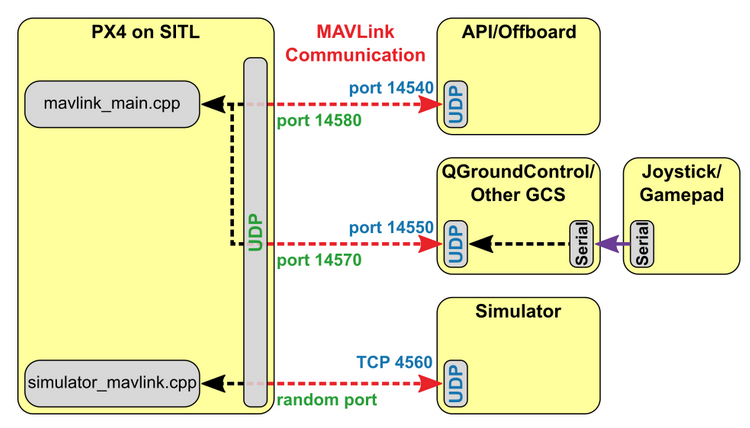
\includegraphics[width=1\linewidth]{../Figures/px4_sitl.png}
        \caption{}
        \label{fig:mavlink_comminication}
    \end{subfigure}
      \hskip 10ex
    \begin{subfigure}[b]{0.26\linewidth}
        \centering
        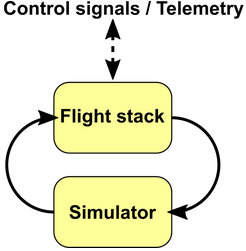
\includegraphics[width=1\linewidth]{../Figures/simulator_mavlink_api.png}
        \caption{}
        \label{fig:simulator_mavlink_api}
    \end{subfigure}
    \caption{Illustrations of the message handling in the SITL simulation environment \cite{px4Autopilot}}
    \label{fig:sitl_simulation_enviroment}
\end{figure}

In Figure \ref{fig:simulator_mavlink_api}, a high level view of the communication between the PX4 flight stack and simulation environment (Gazebo) can be seen. Sensor readings like GPS, IMU data etc. are passed to the PX4 flight controller which returns control outputs (motor actuator commands) to the simulation according to sensor readings. 

The transmission of messages between PX4 and external programs happens using  the user datagram protocol (UDP) ports for MAVLink communication. This is illustrated in Figure \ref{fig:mavlink_comminication}. Here a number of ports are associated to different applications. The UDP Port 14540 is used for offboard control communication which will be python scripts running in the simulation (later on the raspberry pi) for autonomous flight using information from sensors e.g. vision system. The UDP port 14550 is used for communicating with ground control stations (GCS). QgroundControl will be used which offers many features like sensor calibration, radio setup and calibration of transmitters, predefined air frame selection for different drones etc. Moreover, parameters for position and attitude control, speed limits and the like can be changed during flights. However, these parameters can also be changed using ROS in the offboard control script, which will be explained in Section \ref{sec:ros}. The last port, UDP 4560, will be used for transmission of messages between PX4 and the simulation environment.

\todo{Here a link to github can be set regarding how the installation for PX4, gazebo and ROS has been preformed. This have to be done in a REAME file with a bash script which can execute the installation automatically. }

\subsubsection{ROS}
\label{sec:ros}

ROS is an open source software framework to be used in robot applications. This includes a number of libraries and tools with the aim of simplifying the creation of new robotic solutions. Another important feature is the message handling between nodes in the ROS architecture which is visualized in Figure \ref{fig:ros}. The ROS master keeps track on all the nodes in the system an each node goes through registration via the master. Then each node can publish or subscribe to messages which is initiated through the master. This is called topics under the ROS framework and will be used in offboard control where a number of nodes have to communicate to each other.  

\begin{figure}[H]
    \centering
    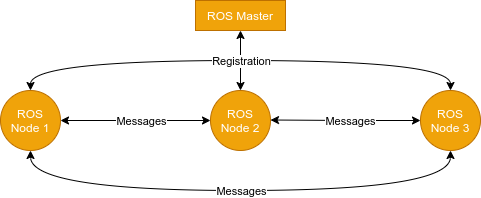
\includegraphics[width=0.6\linewidth]{../Figures/ros.png}
    \caption{Illustrations of a high level view of the architecture in ROS}
    \label{fig:ros}
\end{figure}


\begin{figure}[H]
    \centering
    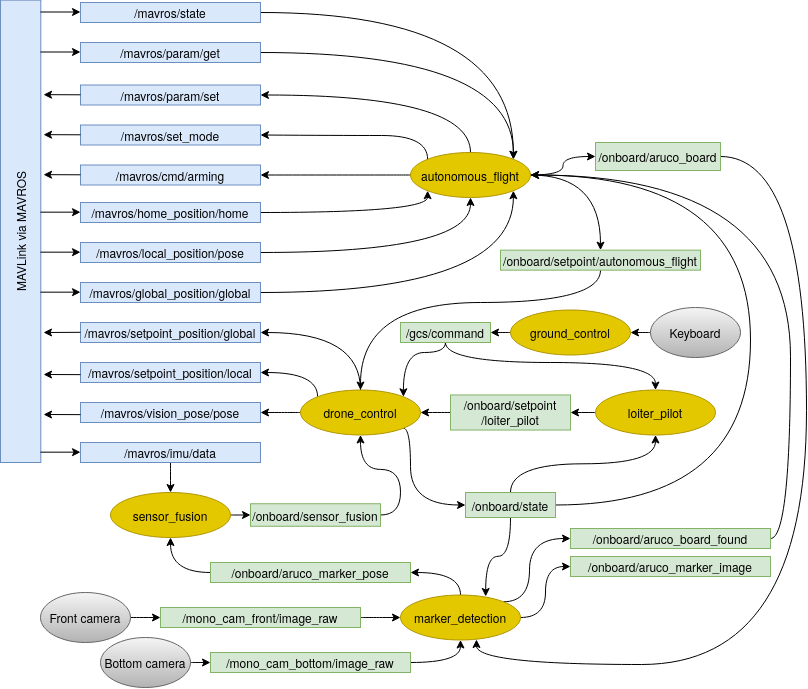
\includegraphics[width=0.95\linewidth]{../Figures/node_communication.png}
    \caption{Illustrations of a high level view of the architecture in ROS}
    \label{fig:ros}
\end{figure}

\begin{table}[H]
\centering
\begin{tabular}{ll}
\hline
\textbf{Keypress} & \textbf{Action}                                    \\ \hline
t                 & drone\_control: Takeoff + offboard + loiter mode         \\
m                 & drone\_control: Mission                                 \\
h                 & drone\_control: Move the drone to home and land         \\
l                 & drone\_control: Switch to loiter control 
\\
k                 & drone\_control: Kill switch
\\
1                 & drone\_control: Estimate aruco pose using front cam 
\\
2                 & drone\_control: Estimate aruco pose using bottom cam 
\\
3                 & drone\_control: Hold position using aruco pose 
\\
wasd              & loiter\_pilot: Forwards, left, back and right respectively           \\
qe                & loiter\_pilot: Rotate left or right (yaw) respectively             \\
zx                & loiter\_pilot: Decrease/increase altitude respectively         
\end{tabular}
\caption{Table of all possible commands from the GCS}
\label{tab:ros_commands}
\end{table}


\subsection{Pose estimation using ArUco markers}
\label{sec:pose_estimation_using_aruco_markers}

\subsection{Sensor fusion for pose optimization}
\label{sec:sensor_fusion_for_pose_optimization}


\end{document}